\documentclass[../calc3.tex]{subfiles}
\graphicspath{{\subfix{../figures/}}}
\begin{document}
\chapter{Three-Dimensional Coordinate Systems}
\section{Vectors in the Plane}
The first goal for calculus 3 is to define the rectangular coordinate plane in 3-space.

In 2-space, this is the normal coordinate axis with coordinates $(x,y)$.

In 3-space, you now have $(x,y,z)$. We have an $xy$-plane, a $yz$-plane, and an $xz$-plane. Also we have octants in 3-space similar to quadrants in 2-space.

The $z$-axis is determined by the right-hand rule: if you curl the fingers on your right hand from the positive $x$-axis to the $y$-axis, your thumb points in the direction of the positive $z$-axis.

\ex Graph $(2,3,4)$.

When graphing points in 3-space, it might be easier to draw a prism to see the three-dimensional components easier.

\ex Graph $(-3,2,-6)$.

In 3-space the distance formula is simliar to 2-space. It is the following:
\[ d=\sqrt{(x_1-x_2)^2+(y_1-y_2)^2+(z_1-z_2)^2} \]

\begin{example}
    Find the distance between $(2,3,4)$ and $(-3,2,-6)$.

    Plug in the numbers into the formula and the answer gives $d=\sqrt{126}$
\end{example}

Similar to circles in 2-space, there are spheres in 3-space. The equation of a sphere is 
\[ (x-x_0)^2+(y-y_0)^2+(z-z_0)^2=r^2 \]

\begin{example}
    Write the equation of a sphere with a diameter having endpoints $(-1,2,1)$ and $(0,2,3)$.

    We can find the center with the midpoint formula, and the center is $(-\frac{1}{2},2,2)$.

    Using the $(-1,2,1)$ endpoint and the center calculated above, we can determine the radius to be $\sqrt{5/4}$.

    Therefore the equation of the sphere is $(x+\frac{1}{2})^2+(y-2)^2+(z-2)^2=\frac{5}{4}$.
\end{example}

\begin{example}
    Find the center and radius of the sphere $x^2+y^2+z^2-2x-4y+8z+17=0$.

    When we complete the square for this, we end up getting $(x-1)^2+(y-2)^2+(z+4)^2=4$.

    Therefore, the center is $(1,2,-4)$ and the radius is $2$.
\end{example}
\pagebreak
\begin{theorem}
    An equation of the form $x^2+y^2+z^2+Gx+Hy+Iz+J=0$ represents a sphere, a point, or has no graph.
\end{theorem}
We would get a point if the radius gives you 0, and if the radius is negative, then there is no graph.

\ex Graph $y=3$ in $\mathbb{R}^3$.

\ex Describe and sketch the surface in $\mathbb{R}^3$ represented by $y=x$.

\ex Graph $x^2+z^2=1$.

\begin{example}
    Describe the graph of $1\leq x^2+y^2+z^2\leq 4$. What if $z\leq 0$?

    This will represent the region between the spheres and centered at the origin with radii of $1$ and $2$. (This is a sphere with center cut out).
    
    The condition $z\leq 0$ will give us a hemisphere, it will only give the lower half of the figure.
\end{example}

\section{Vectors}
\begin{definition}[Vector]
    A vector indicates a quantity that has both magnitude and direction. 

    Examples include displacement, velocity, or force.
\end{definition}
Some ways to notate vectors are $\textbf{u}$, $\overrightarrow{u}$, $\vec{u}$, $\overrightarrow{AB}$, $\vec{AB}$. For the last two of these, these are read as a vector starting at $A$, heading towards $B$.

We say that 2 vectors are equivalent (or equal) if they have the same length and direction.

$0$ vector $(\textbf{0})$ has a length of $0$ and no direction. (Note that $\textbf{0}$ is a vector because it is bolded.)

\begin{definition}[Vector Addition]
    If $\textbf{u}$ and $\textbf{v}$ are positioned so that the initial point of $\textbf{v}$ is at the terminal point of $\textbf{u}$, then $\textbf{u}+\textbf{v}$ is the vector from the initial point of $\textbf{u}$ to the terminal point of $\textbf{v}$.
\end{definition}
Note that $\vec{u}+\vec{v}=\vec{v}+\vec{u}$.

\begin{definition}[Scalar Multiplication]
    If $c$ is a scalar and $\textbf{v}$ is a vector, then $c\textbf{v}$ is the vector whose length is $|c|$ times the length of $\textbf{v}$ and whose direction is the same as $\textbf{v}$ if $c>0$ and is opposite if $c<0$.
\end{definition}

Using the two definitions above, we can find the difference $\textbf{u}-\textbf{v}$. From the above definitions, we can rewrite this as $\vec{u}+(-\vec{v})$, which is equivalent to $\vec{u}-\vec{v}$.

\ex Sketch $\textbf{a}-2\textbf{b}$ and define $\textbf{a}$ and $\textbf{b}$ as you wish.

Coordinate Systems: Generally we place the initial point at the origin and then express a vector as $\textbf{a}=\langle a_1, a_2\rangle$ or $\textbf{a}=\langle a_1,a_2,a_3\rangle$ where $(a_1,a_2)$ 
and $(a_1,a_2,a_3)$ are terminal points.

Given points $A(x_1,y_1)$ and $B(x_2,y_2)$, vector $\textbf{a}=\textbf{AB}$ is $\textbf{a}=\langle x_2-x_1,y_2-y_1\rangle$. (In 3-space the idea is similar.)

\begin{example}
    Express vector $\overrightarrow{P_1P_2}$ in bracket notation if $P_1(1,3)$ and $P_2(4,-2)$.

    Note that we start at the terminal point. Therefore we have $\overrightarrow{P_1P_2}=\langle 4-1,-2-3\rangle=\langle 3,-5\rangle$.

    Note that the vector between the two points and the vector found have the same direction and same length.
\end{example}

Arithmetic Operations: If $\vec{v}=\langle v_1,v_2\rangle$ and $\vec{w}=\langle w_1,w_2\rangle$, then 
\begin{itemize}
    \item $\vec{v}+\vec{w}=\langle v_1+w_1,v_2+w_2\rangle$
    \item $\vec{v}-\vec{w}=\langle v_1-w_1,v_2-w_2\rangle$
    \item $k\vec{v}=\langle kv_1,kv_2\rangle$
\end{itemize}

\begin{example}
    If $\vec{a}=\langle -2,0,1\rangle$ and $\vec{b}=\langle 3,5,-4\rangle$, find $\vec{a}+\vec{b}$ and $\vec{b}-2\vec{a}$.

    Finding $\vec{a}+\vec{b}$ is simple just add them together to get $\langle 1,5,-3\rangle$.

    To find $\vec{b}-2\vec{a}$, multiply $\vec{a}$ by $2$ to get $\langle -4,0,2\rangle$. Then subtracting gives you $\langle 7,5,-6\rangle$.
\end{example}

Properties of Vectors:
\begin{enumerate}
    \item $\vec{a}+\vec{b}=\vec{b}+\vec{a}$
    \item $\vec{a}+(\vec{b}+\vec{c})=(\vec{a}+\vec{b})+\vec{c}$
    \item $\vec{a}+\textbf{0}=\vec{a}$
    \item $\vec{a}+(-\vec{a})=\textbf{0}$ (Additive Inverse)
    \item $c(\vec{a}+\vec{b})=c\vec{a}+c\vec{b}$
    \item $(c+d)\vec{a}=c\vec{a}+d\vec{a}$
    \item $(cd)\vec{a}=c(d\vec{a})$
    \item $1\vec{a}=\vec{a}$
\end{enumerate}

\begin{example}
    Prove property $\#2$ from above.

    Let $\vec{a}=\langle a_1,a_2\rangle$, $\vec{b}=\langle b_1,b_2\rangle$, and $\vec{c}=\langle c_1,c_2\rangle$.

    From the left side of property 2, we have $\langle a_1,a_2\rangle+(\langle b_1,b_2\rangle + \langle c_1,c_2\rangle)$.

    From this, we can simplify to get $\langle a_1+a_2\rangle + \langle b_1+c_1,b_2+c_2\rangle$.

    This gives us $\langle a_1+(b_1+c_1),a_2+(b_2+c_2)\rangle$.

    From the associative law we can rewrite this as $\langle (a_1+b_1)+c_1,(a_2+b_2)+c_2\rangle$.

    This is $\langle a_1+b_1,a_2+b_2\rangle + \langle c_1+c_2\rangle$, which is equivalent to $(\vec{a}+\vec{b})+\vec{c}$. \qed
\end{example}

Unit Vectors: A unit vector is a vector with a length of $1$.

In 2-space, define $\vec{i}=\textbf{i}=\langle 1,0\rangle$ and $\vec{j}=\textbf{j}=\langle 0,1\rangle$ and 3-space, $\vec{i}=\textbf{i}=\langle 1,0,0\rangle$, $\vec{j}=\textbf{j}
=\langle 0,1,0\rangle$, and $\vec{k}=\textbf{k}=\langle 0,0,1\rangle$.

$\vec{i},\vec{j}$, and $\vec{k}$ are called unit or standard basis vectors. All have length 1 and point in the positive direction on the $x-$,$y-$, and $z-$ axes.

For example, $\vec{a}=\langle 1,3,-4\rangle$ can be expressed as $\vec{a}=\vec{i}+3\vec{j}-4\vec{k}$.

\begin{example}
    If $\vec{a}=\vec{i}+2\vec{j}-3\vec{k}$, and $\vec{b}=4\vec{i}+7\vec{k}$, find $2\vec{a}+3\vec{b}$.

    Adding them together gives $14\vec{i}+4\vec{j}+15\vec{k}$.
\end{example}

The norm (or magnitude or length) of a vector is defined as 
\[ |\vec{v}|=||\vec{v}||=\sqrt{v_1^2 + v_2^2} \]

\begin{example}
    Let $\vec{u}=\vec{i}-3\vec{j}+2\vec{k}$ and $\vec{v}=\vec{i}+\vec{j}$. Find: 
    \begin{itemize}
        \item $||\vec{u}||+||\vec{v}||$
        Use the above formula to get $\sqrt{14}+\sqrt{2}$.

        \item $||\vec{u}+\vec{v}||$.
        First add the two vectors to get $\langle 2,-2,2\rangle$. The norm of this is $2\sqrt{3}$.

        \item $\frac{1}{||\vec{v}||}\vec{v}$
        We previously found the magnitude of $\vec{v}$ to be $\sqrt{2}$. So we simply have $\frac{1}{\sqrt{2}}\langle 1,1,0\rangle$. This is $\frac{1}{\sqrt{2}}\vec{i}+\frac{1}{\sqrt{2}}\vec{j}$.
    
        \item $||\frac{1}{||\vec{v}||}\vec{v}||$.
        The norm of $\langle \frac{1}{\sqrt{2}},\frac{1}{\sqrt{2}},0\rangle$ is $1$.
    \end{itemize}
\end{example}
The vector found in the third part of the previous example is known as a unit vector because it has a norm of $1$.

The process of obtaining a unit vector with the same direction is called normalizing $\vec{v}$.

\begin{example}
    Find the unit vector in the direction of $\vec{a}=2\vec{i}-\vec{j}-2\vec{k}$.

    The norm of $a$ is $||\vec{a}|| = \sqrt{4+1+4}=3$. Then normalizing $\vec{a}$ gives $\langle \frac{2}{3},-\frac{1}{3},-\frac{2}{3}\rangle$.
\end{example}

Vectors in Polar Form: Any vector can be written in the following form 
\[ \vec{v}=||\vec{v}||\langle \cos\theta, \sin\theta \rangle \]
We know that $||\vec{v}||$ is the magnitude of the vector and $\langle cos\theta, \sin\theta\rangle$ is the direction.

\begin{example}
    Find the angle that $\vec{v}=\langle -\sqrt{3},1\rangle$ makes with the positive $x$-axis.

    We know we can write this as $\langle -\sqrt{3},1\rangle=||\vec{v}||\langle \cos\theta,\sin\theta\rangle$.

    The magnitude of $\vec{v}$ is $2$, so simplifying a little gives us $\langle -\frac{\sqrt{3}}{2},\frac{1}{2}\rangle=\langle \cos\theta,\sin\theta\rangle$.

     From this, we can see that $\theta$ is the $\theta$ when $\cos\theta = -\frac{\sqrt{3}}{2}$ and $\sin\theta = \frac{1}{2}$. So, $\theta=\frac{5\pi}{6}$.
\end{example}

Forces are often represented by vectors because they have a length and direction. If two forces are applied to the same point, they are concurrent. The two forces together form the resultant force, $\vec{F}_1+\vec{F}_2$.

\begin{example}
    Suppose two forces are applied to an eye bracket. Find the magnitude of the resultant and the angle that it makes with the positive $x$-axis.
    \begin{center}
        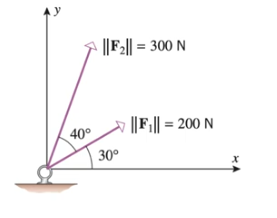
\includegraphics[width=0.5\textwidth]{1.2.1.PNG}
    \end{center}

    From the diagram, we can see that $\vec{F}_1=200\langle \cos 30\degree, \sin 30\degree\rangle = \langle 100\sqrt{3}, 100\rangle$.

    For $\vec{F}_2$, we get $\vec{F}_2=\langle 300\cos 70\degree, 300\sin 70\degree\rangle$.

    Adding them gives $\vec{F}=\langle 100\sqrt{3}+300\cos 70\degree, 100+300\sin 70\degree\rangle$.

    This approximates to $\langle 275.8,381.9\rangle$. The magnitude of this approximates to $||\vec{F}||\approx 471$ N.

    If we let $100\sqrt{3}+300\cos 70\degree$ be $||\vec{F}||\cos\theta$, then we can determine the angle. 

    When we find $\theta$ in $\cos\theta = \frac{100\sqrt{3}+300\cos 70\degree}{471}$, we get $\theta \approx 54.2\degree$.
\end{example}

\begin{example}
    A 100-lb weight hangs from two wires. Find the forces (tensions) $\vec{T}_1$ and $\vec{T}_2$ in both wires and the magnitude of those tensions.
    \begin{center}
        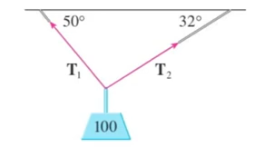
\includegraphics[width=0.5\textwidth]{1.2.2.PNG}
    \end{center}

    Note that $\vec{T}_1$ does not have an angle of $50\degree$, rather it has a degree of $130\degree$ from the point.

    Therefore, we have $\vec{T}_1=|\vec{T}_1|\langle \cos 130\degree, \sin 130\degree\rangle$.

    Note we can rewrite this with to be in the first quadrant as $|\vec{T}_1|\langle -cos 50\degree, \sin 50\degree\rangle$.

    We also have $\vec{T}_2=|\vec{T}_2|\langle \cos 32\degree, \sin 32\degree\rangle$.

    We also see that the weight of the block is $\vec{W}=100\langle 0,-1\rangle = \langle 0,-100\rangle$, so we see to balance this out, both tension forces need to equal $\langle 0,100\rangle$.

    Therefore, we see that $-|\vec{T}_1|\cos 50\degree + |\vec{T}_2|\cos 32\degree = 0$ (addition of the $\vec{i}$ components).

    We also have $|\vec{T}_1\sin 50\degree + |\vec{T}_2|\sin 32\degree = 100$ ($\vec{j}$ components).

    Solving for $|\vec{T}_1|$ and $|\vec{T}_2|$ from this gives us $85.64$ lbs and $64.91$ lbs respectively.

    Plugging these values back in gives us the tension vectors. 

    $\vec{T}_1 \approx \langle -55.05, 65.60\rangle$

    $\vec{T}_2 \approx \langle 55.05, 34.40 \rangle$
\end{example}

\section{The Dot Product}
\begin{definition}[The Dot Product]
    If $\vec{a}=\langle a_1,a_2,a_3\rangle$ and $\vec{b}=\langle b_1,b_2,b_3\rangle$, then the dot product $\vec{a}\cdot \vec{b}$ is 
    \[ \vec{a}\cdot \vec{b} = a_1b+1+a_2b_2+a_3b_3 \]
    This is called the scalar or inner product. (Note: 2-space is a similar idea)
\end{definition}

\begin{example}
    $(\vec{i}+2\vec{j}-3\vec{k})\cdot (2\vec{j}-\vec{k})$

    Using the dot product formula gives you $7$.
\end{example}

Properties of dot products:
\begin{enumerate}
    \item $\vec{a}\cdot \vec{a} = |\vec{a}|^2$
    \item $\vec{a}\cdot \vec{b} = \vec{b}\cdot \vec{a}$
    \item $\vec{a}\cdot (\vec{b}+\vec{c})=\vec{a}\cdot \vec{b}+\vec{a}\cdot \vec{c}$
    \item $(c\vec{a})\cdot \vec{b}=c(\vec{a}\cdot \vec{b})=\vec{a}\cdot (c\vec{b})$
    \item $\vec{0}\cdot \vec{a}=0$
\end{enumerate}

\begin{example}
    Prove the first property from above.

    Let $\vec{a}=\langle a_1,a_2,a_3\rangle$.

    The dot product of $\vec{a}$ and $\vec{a}$ gives us $a_1^2+a_2^2+a_3^2$.

    The magnitude of this is $\sqrt{a_1^2+a_2^2+a_3^2}^2$ which is equal to $|\vec{a}|^2$ \qed
\end{example}

\begin{example}
    Prove the third property from above.

    Let $\vec{a}=\langle a_1,a_2,a_3\rangle$, likewise for $\vec{b}$ and $\vec{c}$.

    Then when we do $\vec{a}\cdot (\vec{b}+\vec{c})$ we get 
    \begin{align*}
        \langle a_1,a_2,a_3\rangle \cdot (\langle b_1,b_2,b_3\rangle + \langle c_1,c_2,c_3\rangle)\\
        = \langle a_1,a_2,a_3\rangle \cdot \langle b_1+c_1, b_2+c_2, b_3+c_3\rangle\\
        = a_1(b_1+c_1)+a_2(b_2+c_2)+a_3(b_3+c_3)\\
        = a_1b_1+a_1c_1+a_2b_2+a_2c_2+a_3b_3+a_3c_3\\
        = (a_1b_1+a_2b_2+a_3b_3)+(a_1c_1+a_2c_2+a_3c_3)\\
        = \vec{a}\cdot \vec{b}+\vec{a}\cdot \vec{c} 
    \end{align*}\qed 
\end{example}
\pagebreak
\begin{theorem}
    $\vec{a}\cdot \vec{b}=|\vec{a}||\vec{b}|\cos\theta$, where $\theta$ is the angle between $\vec{a}$ and $\vec{b}$.
\end{theorem}
\begin{corollary}
    $\cos\theta = \frac{\vec{a}\cdot \vec{b}}{|\vec{a}||\vec{b}|}$
\end{corollary}

\begin{example}
    Find the angle between $\vec{u}=\vec{i}-2\vec{j}+2\vec{k}$ and $\vec{v}=-3\vec{i}+6\vec{j}+2\vec{k}$.

    The dot product of the two gives $-11$.

    The magnitude of $\vec{u}$ is $3$ and the magnitude of $\vec{v}$ is $7$.

    We see that $\cos\theta = -\frac{11}{3\cdot 7}$, so $\theta = 2.12$ radians or $121.6\degree$.
\end{example}

Recall, $\vec{a}\cdot \vec{b}=|\vec{a}||\vec{b}|\cos\theta$. Since $|\vec{a}||\vec{b}|$ is always positive, the sign of the dot product is determined by $\cos\theta$.
\begin{itemize}
    \item If $\vec{a}\cdot \vec{b}>0$, then the angle is acute.
    \item If $\vec{a}\cdot \vec{b}<0$, then the angle is obtuse.
    \item If $\vec{a}\cdot \vec{b}=0$, then the vectors are orthogonal.
\end{itemize}

To determine if two vectors are parallel, the vectors have to be scalar multiples of each other.

\begin{definition}[Direction Angles]
    The direction angles $\alpha$, $\beta$, and $\gamma ([0,\pi])$ are the angles that $\vec{a}$ makes with the positive $x-$, $y-$, and $z-$ axes. Their cosines are called direction cosines.
\end{definition}
$\cos\alpha = \frac{\vec{a}\cdot \vec{i}} \implies \cos\alpha = \frac{a_1}{|\vec{a}|}$. Likewise, $\cos\beta = \frac{a_2}{|\vec{a}|}$ and $\cos\gamma = \frac{a_3}{|\vec{a}|}$.

Notice that $\cos^2\alpha + \cos^2\beta + \cos^2\gamma = 1$.

Also $\vec{a}=|\vec{a}|\langle \cos \alpha, \cos\beta, \cos\gamma \rangle$, which can be expressed as $\frac{\vec{a}}{|\vec{a}|}=\langle \cos\alpha, \cos\beta, \cos\gamma\rangle$.

So, the direction cosines form the unit vector in the direction of $\vec{a}$.

\begin{example}
    Find the direction cosines of $\vec{a}=\langle 2,-4,4\rangle$ and approximate the direction angles to the nearest degree.

    The magnitude of $\vec{a}$ is $6$.

    From the formulas, we can find that $\cos\alpha = \frac{1}{3}$, $\cos\beta = -\frac{2}{3}$, and $\cos\gamma = \frac{2}{3}$.

    Finding the angles gives us $\alpha \approx 71\degree$, $\beta \approx 132\degree$, and $\gamma \approx 48\degree$.
\end{example}

\begin{example}
    Find the angle between a diagonal of a cube and one of its edges.

    Let's call the vector from the diagonal to the edge as $\vec{d}$ and the length of the edge be $a$.

    We get $\vec{d}=\langle a,a,a\rangle$ as a result. The magnitude of $\vec{a}$ ends up being $\sqrt{3a^2}$.

    We get that $\cos\alpha = \frac{a}{\sqrt{3a^2}}=\frac{1}{\sqrt{3}}$.

    This approximates $\alpha \approx 0.955$ radians or $54.7\degree$.
\end{example}

proj$_{\vec{a}}\vec{b}$ is the vector projection of $\vec{b}$ onto $\vec{a}$

comp$_{\vec{a}}\vec{b}$ is the scalar projection of $\vec{b}$ onto $\vec{a}$ (a signed magnitude of the vector projection).

If we look at the scalar projection, comp$_{\vec{a}}\vec{b}=|\vec{b}|\cos\theta$ and remember that $\cos\theta = \frac{\vec{a}\cdot\vec{b}}{|\vec{a}||\vec{b}|}$.
Therefore comp$_{\vec{a}}\vec{b}=\frac{\vec{a}\cdot \vec{b}}{|\vec{a}|}$.

The projection will just be the magnitude (which is the scalar projection) multiplied by the unit vector: $\frac{\vec{a}\cdot \vec{b}}{|\vec{a}|}\left(\frac{\vec{a}}{|\vec{a}|}\right)$.

This is equal to $\frac{\vec{a}\cdot \vec{b}}{|\vec{a}|^2}\vec{a}$.

\begin{example}
    Find the scalar and vector projections of $\vec{b}=\langle 1,1,2\rangle$ onto $\vec{a} = \langle -2,3,1\rangle$.

    The dot product of the vectors is $3$, the magnitude of $\vec{a}=\sqrt{14}$.

    From the formula above, the scalar projection is $\frac{3}{\sqrt{14}}$.

    The vector projection gives $\frac{3}{(\sqrt{14})^2}\langle -2,3,1\rangle$, simplifying to $\langle -\frac{3}{7},\frac{9}{14},\frac{3}{14} \rangle$.
\end{example}

Previously, you learnt work is defined as $W=F\cdot d$ (this only applies when the force is directed along the line of motion).

Now we can define work as $W=(|\vec{F}|\cos\theta)|\vec{d}|$. Moving stuff around gives $W=|\vec{F}||\vec{D}|\cos\theta$.

Now we see that $W=\vec{F}\cdot \vec{d}$. (Work is constant which means it should result in a scalar.)

\begin{example}
    A wagon is pulled horizontally by exerting a constant force of 10 lb on the handle at an angle of $60\degree$ with the horizontal. How much work is done in moving the wagon 50 feet?

    We can easily see that the displacement vector is $\vec{d}=\langle 50,0\rangle$.

    The force vector we must divide into components, so we get $\vec{F}=10\langle \cos 60\degree, \sin 60\degree\rangle = \langle 5,5\sqrt{3}\rangle$.

    So the dot product of both vectors gives us $250$ ft-lb.
\end{example}

\end{document}